\chapter{Introduction}

Our objective is to develop a computational environment for the exploration
of parametric polytopes. A computational environment is one in which
we can apply rigorous definitional constraints on symbolic constructions, and
likewise manipulate them to reveal properties that may be of interest.
A parametric polytope is the union of two concepts. The first is the idea
of parameters, which are our unknown constraints in a system. The second
is a polytope, which is a some what geometric construction. We will
build an intuition of a polytope in this section, and formally define it
in the next chapter. Parameters will be applied in the computation realm
and are expanded in Section 3.


\section{A Geometric Intuition of a Polytope}

A polytope is a geometrically realizable graph composed
of linearly connected vertices\cite{Coxeter}.
A ``graph" is meant in the combinatorial sense of a structure composed of
vertices and edges that show connectivity. Thus a geometric realization
of a graph with linearly connected vertices is highly analogous to how we would traditionally
draw a graph. Figure \ref{fig:graph} shows a graph in with vertices labeled
with numbers and edges between them.

\begin{figure}[h!]
  \centering
    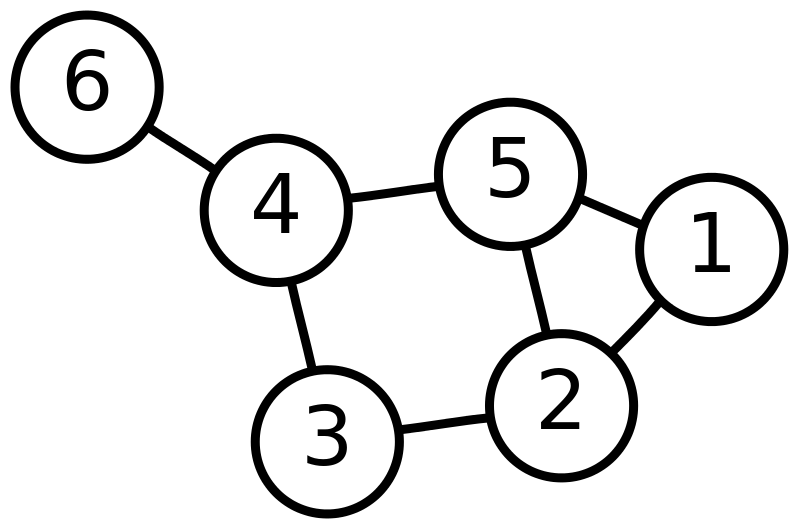
\includegraphics[width=0.5\textwidth]{img/6graph.png}
  \caption{An example of a graph.}
  \label{fig:graph}
\end{figure}

The informal term ``flat" implies the path between two vertices
on our polytope are connected by line segments. Thus for something to be
considered geometrically realizable, we must be able to assign tuple values
to the vertices. An N-polytope then exists in the corresponding euclidean
space dimension. For our purposes we will primarily use the real numbers,
$\mathbb{R}^N$, for an N-polytope.

Figure \ref{fig:polygons}
shows a two dimensional polytope, more commonly
known as a polygon. The polgons we will primarily consider are 1-cycle
graphs. 1-cycle implies that given any point there exist one path that exits
then returns to the starting point.
In three dimensions, polytopes are commonly known as a polyhedra.
Figure \ref{fig:polyhedra} shows a polyhedral representation of a dolphin.
Using this picture as reference, we see that given a vertex on a polyhedra
there may be
multiple cycles, or paths that exit then return to the vertex.
Thus many assumptions about the properties of polytopes are contingent upon
their dimensionality.
Polytopes may have properties of convexity,
connectedness,
and closure associated with them. In order to study these properties
we will elucidate a combinatoric and geometric representation
in the coming sections. More importantly we will do so rigorously!
These representations are somewhat distinct and we will see the
implications as we later develop a computational type framework.

\begin{figure}[h!]
  \centering
    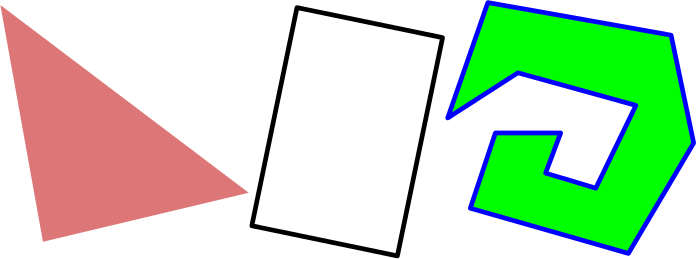
\includegraphics[width=0.75\textwidth]{img/assorted_polygons.png}
  \caption{Polygons, or two dimensional polytopes}
  \label{fig:polygons}
\end{figure}

\begin{figure}[h!]
  \centering
    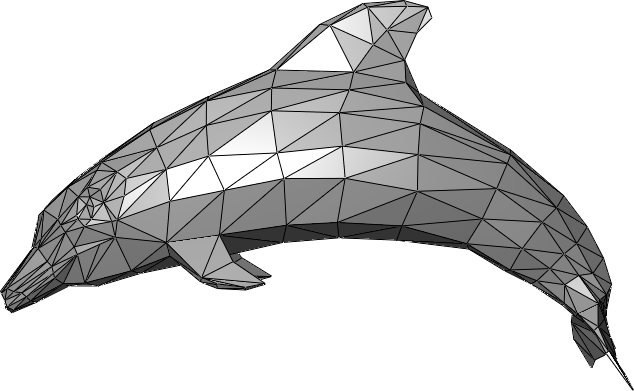
\includegraphics[width=0.75\textwidth]{img/Dolphin_triangle_mesh.png}
  \caption{A polyhedral representation of a dolphin, or a three dimensional polytope}
  \label{fig:polyhedra}
\end{figure}

\section{Flexibility of Polyhedra}

Our initial problem comes via the flexibility of polyhedra. In order to
understand flexibility of polyhedra it may be easier first to introduce the
concept of rigidity. In this case we will be concerned with 3-dimensional
polytopes, polyhedra, and observing the shape of the faces. If we give each
edge (connection between vertices) a fixed length and the freedom to pivot
around the vertex, a rigid polyhedra will not be able to deform. Cauchy's
Ridgidity theorem proves this for any convex polyhedra\cite{Gluck_1975}.
If we allow the same degrees of freedom on the edges and the shape of the
faces does not change it is called \emph{flexible}\cite{Connelly_1977}.

In 2015 Maria Hempel presented an analysis of this problem using a representation
of a polyhedra with edges and faces specified via angles and lengths
\cite{Hempel_2015}.
Such representations may be useful in a variety of disciplines, but our
focus will be strictly structural and for enhancing the foundations for
discovering flexible polyhedra.
We will expand on the significance of this representation in later sections.

\section{Personal Perspective}

This section will outline the personal motivation for this project.
In 2009 I first became interested with 3D printing. One of the
key promises of 3D printing is localized and personalized production.
This very quickly lead me into the world of generative geometry and in
particular OpenSCAD. OpenSCAD is a solid modeling application which
generates solids from scripts. Generative geometry from software allows
ua designer to expose parameters for a user to manipulate, thus allowing
many designs to be created from one structure and a user to make a solid
that fits their unique needs or ecology. Many in this space call
such a process "appropriate design".

One notable difficulty of OpenSCAD is that it includes its own
programming language.
In search of deeper understanding I began to work on my own replacements
for OpenSCAD. In 2013 this began with the TextCAD project, which allowed
one to use the principles of Object Oriented Programming (OOP) via Python.
Concurrently, Christopher Olah was working on ImplicitCAD, a pure
Haskell implementation of a solid modeller. I had realized that TextCAD
had solved, to some extent, the expressibility issue with OpenSCAD but
did not solve the complexity issue. Christopher Olah and I were on
parallel paths with the expressibility issue, but he had approached
the problem from a mathematical perspective of functionally defined
solids. In fact, Haskell is a functional language which made this approach
intrinsic. After spending some time testing TextCAD, I discovered
the principles of OOP to be insufficient for correct representations
of solids. One of the key insights made by Christopher was the importance
of maintaining functional definitions of solids.

I strongly felt that one of the balances a good generative modeller should
possess is readability. Many functional languages, including Haskell and
Lisp are difficult for someone to parse. OpenSCAD may read very similar
to a markup langauge.
For a year TextCAD
sat until I heard about Julia. I began to use it as a replacement for
MATLAB, but quickly realized it has all the requirements to be a
functional programming language. This lead me to contribute to the
geometry ecosystem in hopes of developing a solid modeling framework.
Later in 2014 I was recruited by the Lewis Group
at Harvard University to develop a path planner for 3D printers, and
later took a position at their spin-off company Voxel8 to continue my work.
This afforded me the opportunity to spend most of my time researching and
writing computational geometry software on polygonal meshes and
polygons.

After leaving Voxel8 I began to pursue my work on solid modeling again.
One of the most apparent issue was how to increase performance and
propagate parameters in the model.
The requirements laid out for computing the flexibility
problem were parallel to my challenges. Much of my work in the middle of 2015
was collaborating with people working in the visualization space, so I
had a good understanding of polygonal meshes. My hope was that I could
make a contribution to this problem in the computational realm. Of course
much of this work is nascent and I hope the structure of the
data and packages will provide a good base for projects to come.
It builds on much of what I have learned in the past 5 years of research
into computational geometry.
One notable absence from this report is the progress made in the
functional representation of solids. Especially towards the convergence of
combinatorial and functional polytopes. This work is embedded in the
packages we used for this project, and some of the possibilities will
be discussed in the conclusion.




